\documentclass[tikz,border=1.618]{standalone}
\usetikzlibrary{3d,perspective}

% dimensions
\def\r{1}  % radius
\def\w{6.5}% width
\def\h{3.5}% height

% styles
\tikzset{my orange/.style={fill=orange!#1}}

\begin{document}
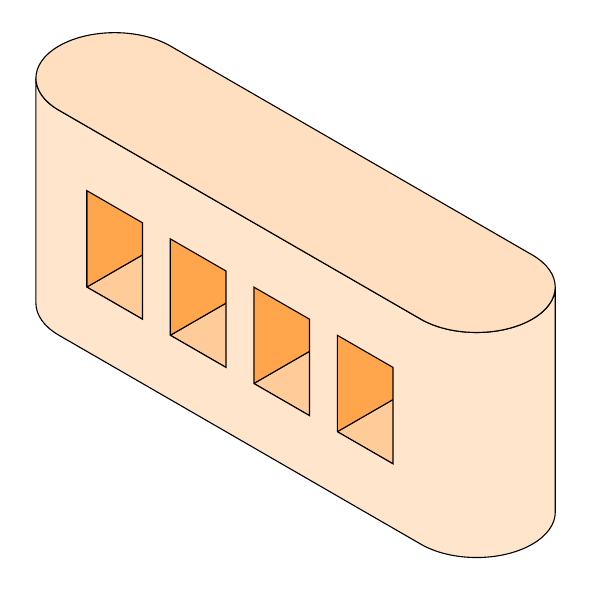
\begin{tikzpicture}[isometric view,rotate around z=180]
% holes
\foreach\i in {0.5,2,3.5,5}
{
  \draw [canvas is xy plane at z=1 ,my orange=40] (\r,\i) rectangle (-\r,\i+1);
  \draw [canvas is xz plane at y=\i,my orange=70] (\r,1)  rectangle (-\r,\h-1);
}
% front surface
\draw[even odd rule,my orange=20]
   (-45:\r) arc (-45:0:\r) --++ (0,\w)  arc (0:135:\r) --++
   (0,0,\h) arc (135:0:\r) --++ (0,-\w) arc (0:-45:\r) -- cycle
   [canvas is yz plane at x=\r] (0.5,1) rectangle (1.5,\h-1)
                                (2  ,1) rectangle (3  ,\h-1) 
                                (3.5,1) rectangle (4.5,\h-1)
                                (5  ,1) rectangle (6  ,\h-1);
% top surface
\draw[canvas is xy plane at z=\h,my orange=25]
   (-180:\r) arc (-180:0:\r) --++ (0,\w)  arc (0:180:\r) -- cycle;
\end{tikzpicture}
\end{document}